\subsubsection{Insertion}

In description and figure \ref{fig:algorithm:real:example} have already mentioned some of the flow of insertion, so in here will show the table if insert another value into the table. Insert $\pi (3.14159)$ into table, which will become like figure \ref{fig:algorithm:real:insertion:example}.

\begin{figure}[h]
\centering
%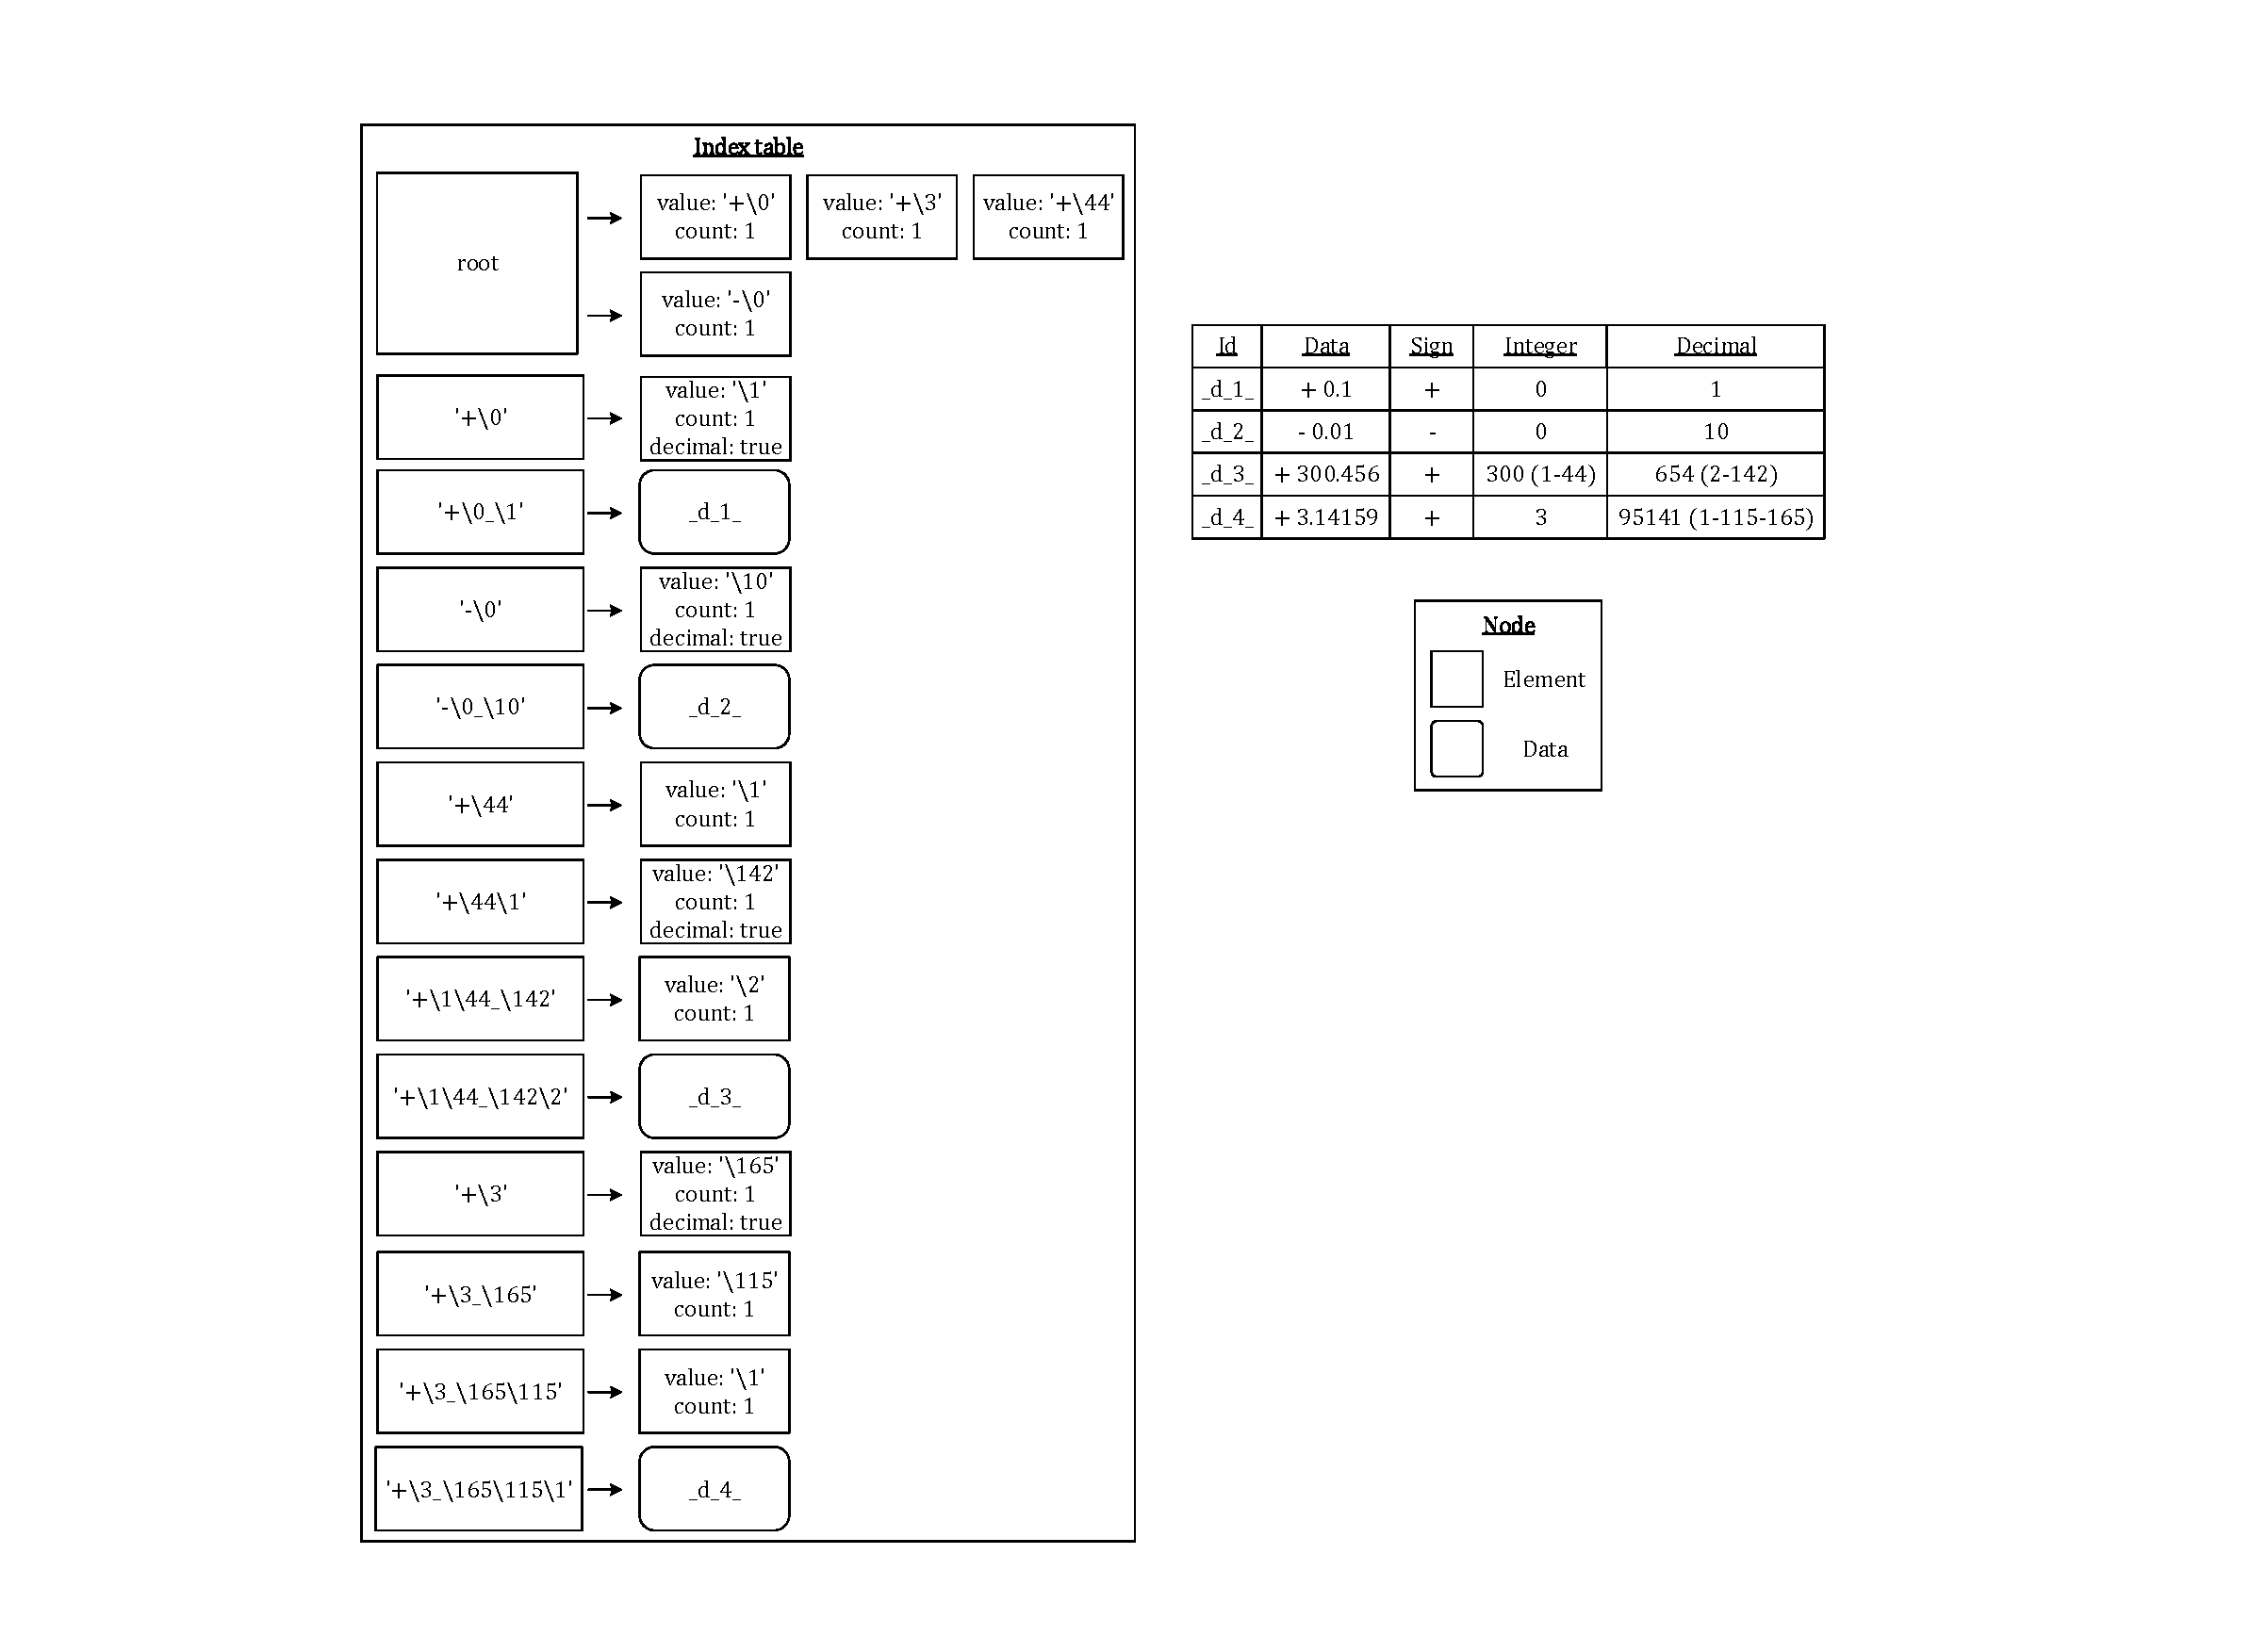
\includegraphics[scale=0.45]{./algorithm/real/pic/insertion/example_v4.png}
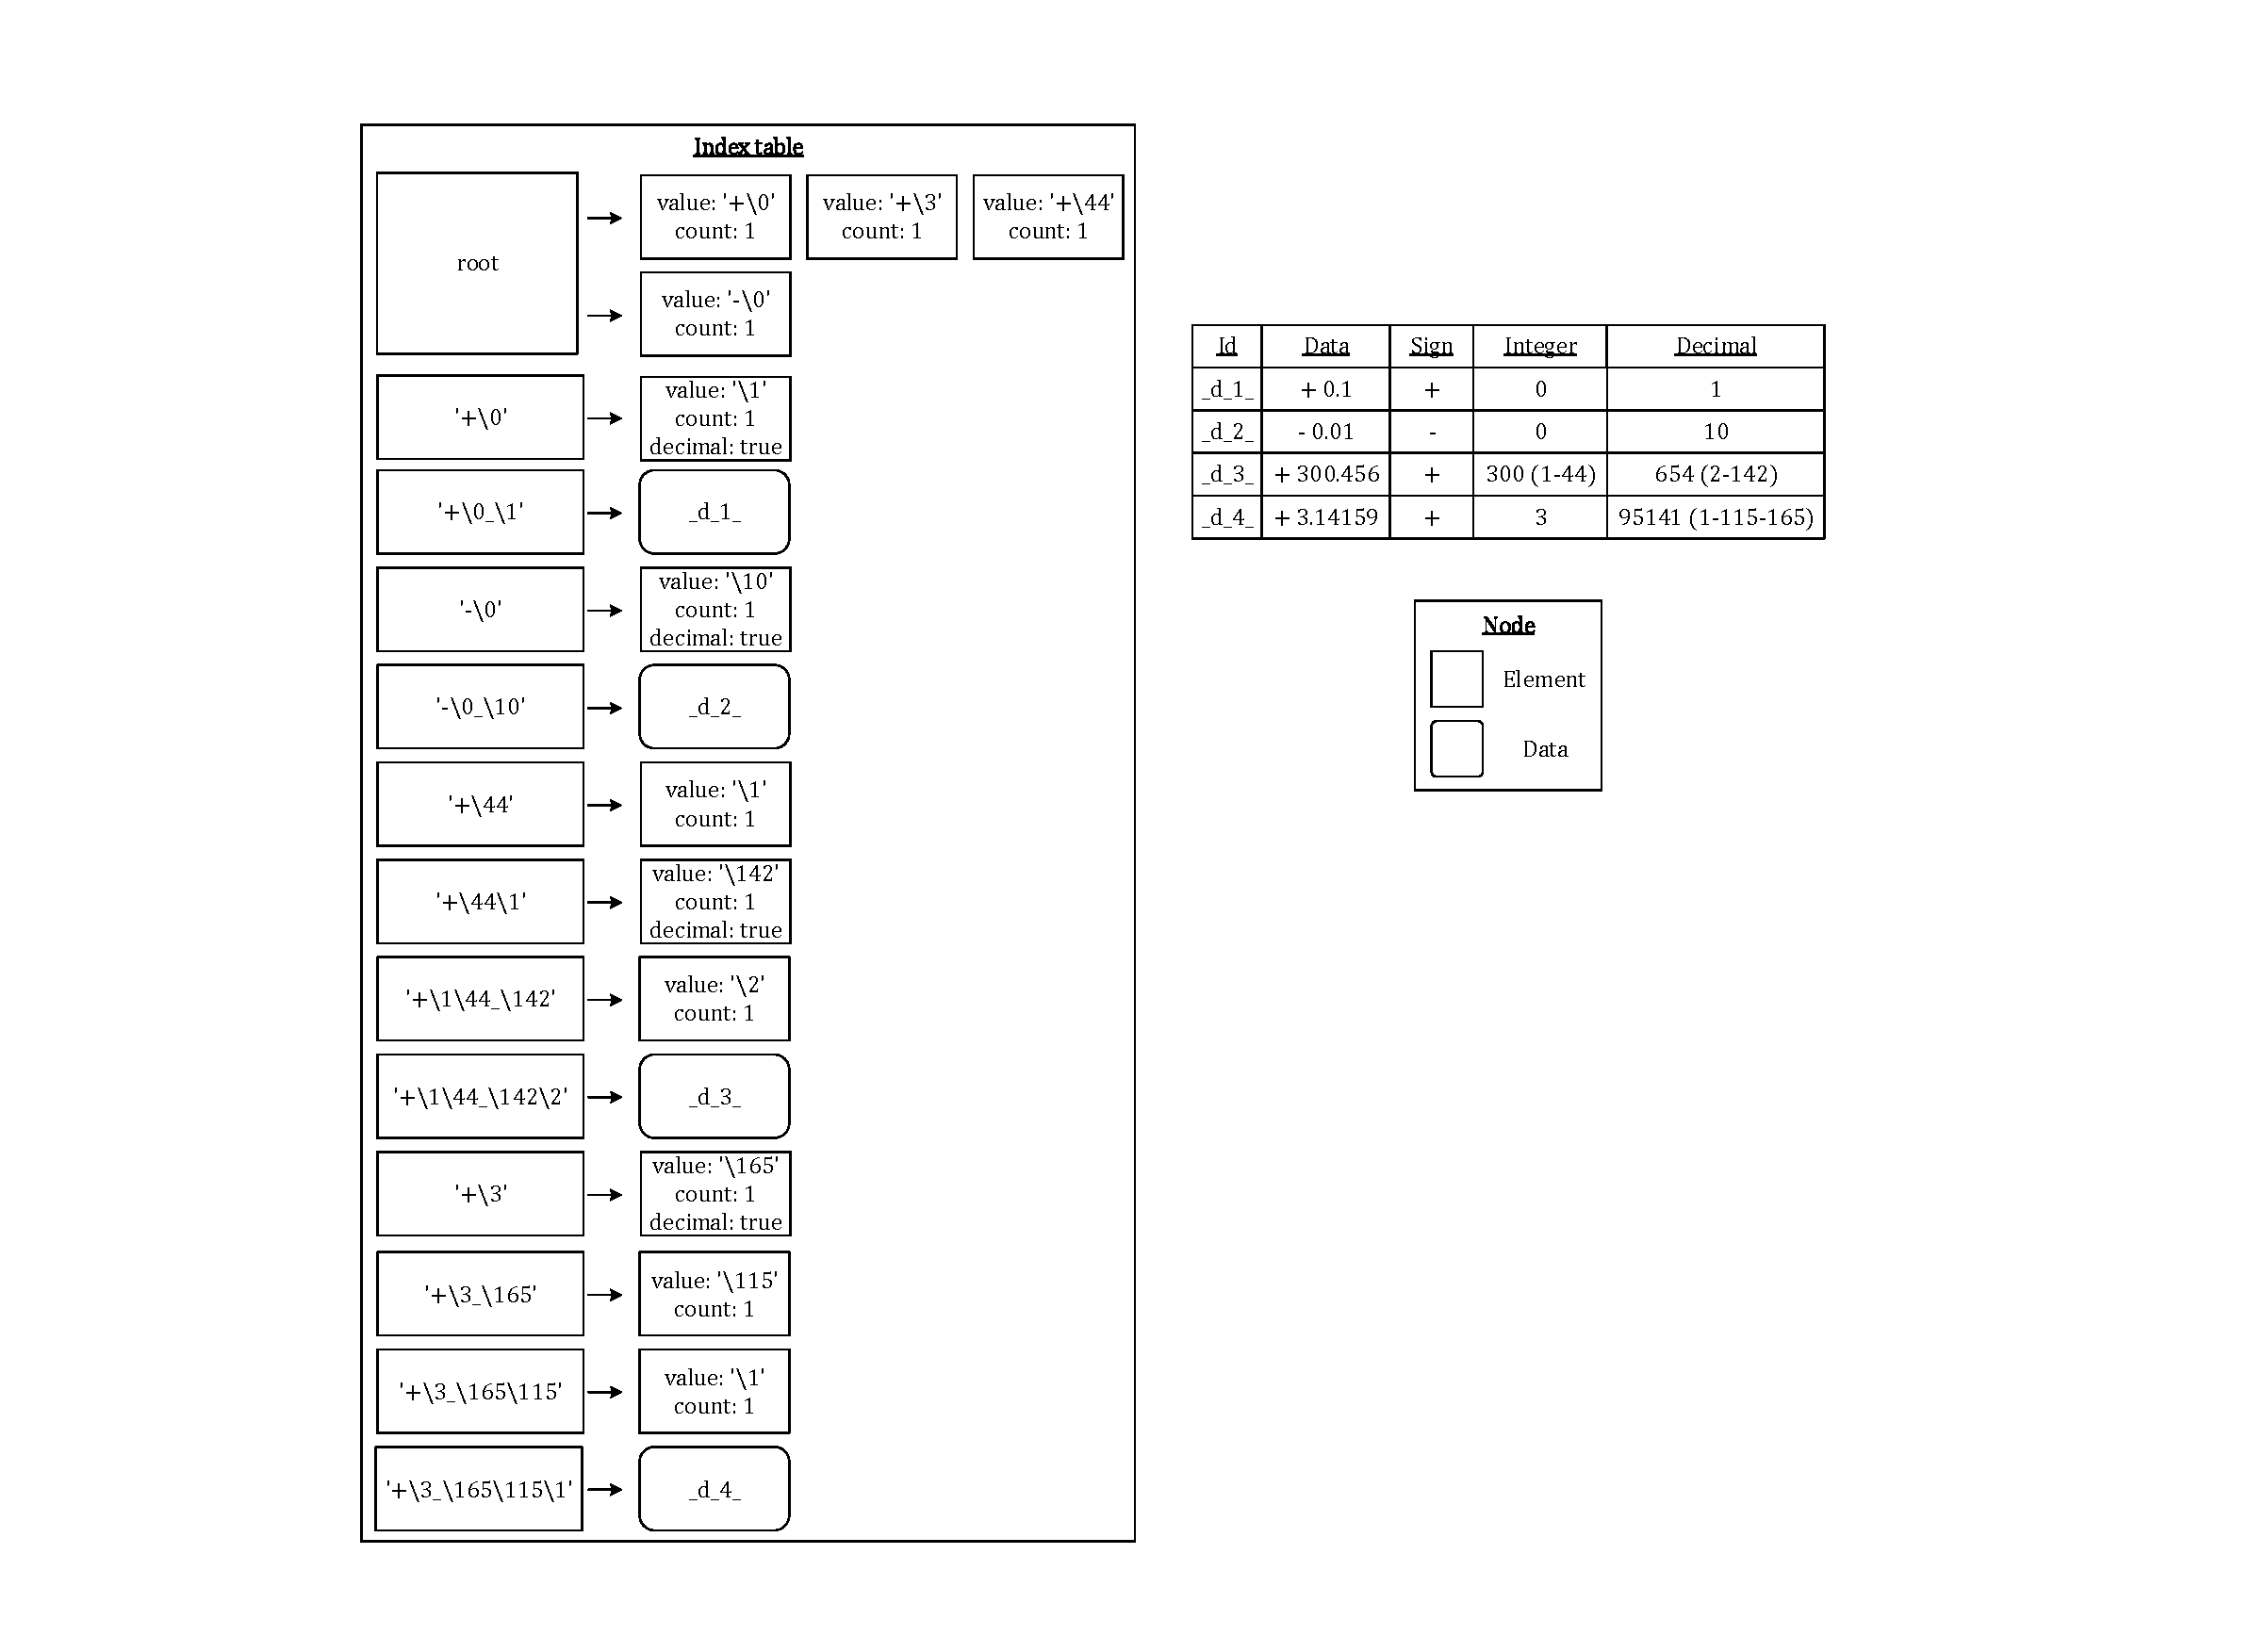
\includegraphics[width=0.8\textwidth]{./algorithm/real/pic/insertion/example_v4.pdf}
\caption{The table after inserted $\pi (3.14159)$.}
\label{fig:algorithm:real:insertion:example}
\end{figure}

Figure \ref{fig:algorithm:real:insertion:example} shows that the $\pi (+3.14159)$ is store the value by its \textit{"Sign"} $(+)$, \textit{"Integer"} $(3)$ and \textit{"Decimal"} $(95141)$.

The \textit{"Sign"} is pointing the last byte of the \textit{"Integer"}, the reason of point to the last byte is because of the dynamic length of \textit{REAL}, also assume the the byte of the data is longer than the input byte length:

\begin{enumerate}

\item  If the \textit{"Sign"} is pointing the first byte, then when we search the result for the input, this may need to compare more byte or we need to get the whole \textit{"Integer"} in the worst case to sure that this value is suitable or not to the input.

\item If \textit{"Sign"} is pointing the last byte, then we just need to compare few bytes or the same byte length of the input that we can immediately to know that is a result or not. So this indexing can speed up the searching.

\end{enumerate}

Time complexity should be $O(b!)$ which domain as $O(b)$, and $b$ is the length of the byte needed where $b = 4$ in this case.

